
%(BEGIN_QUESTION)
% Copyright 2011, Tony R. Kuphaldt, released under the Creative Commons Attribution License (v 1.0)
% This means you may do almost anything with this work of mine, so long as you give me proper credit

This level-control system appears to have a problem.  The SP is set for 2.5 feet (out of a 0-5 foot range), and the PV display on the controller faceplate registers 2.49 feet.  A field operator informs you that a sightglass on this vessel reads 3 feet 9 inches, and the control valve stem position is approximately 60\% open.

$$\includegraphics[width=15.5cm]{i03399x01.eps}$$

\vskip 10pt

Identify the likelihood of each specified fault for this control system.  Consider each fault one at a time (i.e. no coincidental faults), determining whether or not each fault could independently account for {\it all} measurements and symptoms in this circuit.

% No blank lines allowed between lines of an \halign structure!
% I use comments (%) instead, so that TeX doesn't choke.

$$\vbox{\offinterlineskip
\halign{\strut
\vrule \quad\hfil # \ \hfil & 
\vrule \quad\hfil # \ \hfil & 
\vrule \quad\hfil # \ \hfil \vrule \cr
\noalign{\hrule}
%
% First row
{\bf Fault} & {\bf Possible} & {\bf Impossible} \cr
%
\noalign{\hrule}
%
% Another row
LT out of calibration (outputting wrong current) &  &  \cr
%
\noalign{\hrule}
%
% Another row
LIC input out of calibration (not interpreting signal properly) &  &  \cr
%
\noalign{\hrule}
%
% Another row
LIC output out of calibration (not sending correct mA signal to I/P) &  &  \cr
%
\noalign{\hrule}
%
% Another row
I/P out of calibration (not outputting correct pressure) &  &  \cr
%
\noalign{\hrule}
%
% Another row
LIC is poorly tuned (not making good control ``decisions'') &  &  \cr
%
\noalign{\hrule}
} % End of \halign 
}$$ % End of \vbox

\underbar{file i03399}
%(END_QUESTION)





%(BEGIN_ANSWER)

% No blank lines allowed between lines of an \halign structure!
% I use comments (%) instead, so that TeX doesn't choke.

$$\vbox{\offinterlineskip
\halign{\strut
\vrule \quad\hfil # \ \hfil & 
\vrule \quad\hfil # \ \hfil & 
\vrule \quad\hfil # \ \hfil \vrule \cr
\noalign{\hrule}
%
% First row
{\bf Fault} & {\bf Possible} & {\bf Impossible} \cr
%
\noalign{\hrule}
%
% Another row
LT out of calibration (outputting wrong current) & $\surd$ &  \cr
%
\noalign{\hrule}
%
% Another row
LIC input out of calibration (not interpreting signal properly) & $\surd$ &  \cr
%
\noalign{\hrule}
%
% Another row
LIC output out of calibration (not sending correct mA signal to I/P) &  & $\surd$ \cr
%
\noalign{\hrule}
%
% Another row
I/P out of calibration (not outputting correct pressure) &  & $\surd$ \cr
%
\noalign{\hrule}
%
% Another row
LIC is poorly tuned (not making good control ``decisions'') &  & $\surd$ \cr
%
\noalign{\hrule}
} % End of \halign 
}$$ % End of \vbox

%(END_ANSWER)





%(BEGIN_NOTES)

{\bf This question is intended for exams only and not worksheets!}

%(END_NOTES)


